% MIT License

% Copyright (c) 2022 Chiyuru

% Permission is hereby granted, free of charge, to any person obtaining a copy of this software and associated documentation files (the "Software"), 
% to deal in the Software without restriction, including without limitation the rights
% to use, copy, modify, merge, publish, distribute, sublicense, and/or sell
% copies of the Software, and to permit persons to whom the Software is
% furnished to do so, subject to the following conditions:

% The above copyright notice and this permission notice shall be included in all copies or substantial portions of the Software.

% THE SOFTWARE IS PROVIDED "AS IS", WITHOUT WARRANTY OF ANY KIND, EXPRESS OR IMPLIED, INCLUDING BUT NOT LIMITED TO THE WARRANTIES OF MERCHANTABILITY,
% FITNESS FOR A PARTICULAR PURPOSE AND NONINFRINGEMENT. IN NO EVENT SHALL THE AUTHORS OR COPYRIGHT HOLDERS BE LIABLE FOR ANY CLAIM, DAMAGES OR OTHER
% LIABILITY, WHETHER IN AN ACTION OF CONTRACT, TORT OR OTHERWISE, ARISING FROM,
% OUT OF OR IN CONNECTION WITH THE SOFTWARE OR THE USE OR OTHER DEALINGS IN THE SOFTWARE.

\documentclass[UTF8]{ctexart}

\usepackage{amsmath}
\usepackage{cases}
\usepackage{cite}
\usepackage{graphicx}
\usepackage[margin=1in]{geometry}
\usepackage{float}
\geometry{a4paper}
\usepackage{fancyhdr}
\usepackage{multirow}
\usepackage{listings}
\pagestyle{fancy}
\fancyhf{}


\title{ICS-lab3实验报告}
\author{孔浩宇 PB20000113}
\date{\today}
\pagenumbering{arabic}

\begin{document}

\fancyhead[L]{孔浩宇}
\fancyhead[C]{ICS-lab3实验报告}
\fancyfoot[C]{\thepage}

\maketitle
\tableofcontents
\newpage

\section{实验目的}
    对于一个储存在从x3101开始的连续的内存位置的、长度为N的字符串,
    求出其最长的连续重复字符子串的长度,并将结果存储在x3050中.

\section{实验原理}
    \subsection{实现if语句}
    \begin{enumerate}
        \item [(1)]if A==B.
        \begin{lstlisting}[basicstyle=\ttfamily,language={[x86masm]Assembler}]
                ADD     R, A, #0
                NOT     R, R
                ADD     R, R, #1    ; R=-A
                ADD     R, R, B     ; R=B-A
                BRnp     AFTER      ;
                ...                 ; if(B-A==0) do this
            AFTER                   
        \end{lstlisting}

        \item [(2)]if A>B.
        \begin{lstlisting}[basicstyle=\ttfamily,language={[x86masm]Assembler}]
            ADD     R, A, #0
            NOT     R, R
            ADD     R, R, #1    ; R=-A
            ADD     R, R, B     ; R=B-A
            BRzp     AFTER      ;
            ...                 ; if(B-A<0) do this
        AFTER                   
        \end{lstlisting}

        \item [(3)]if A$\geq$B.
        \begin{lstlisting}[basicstyle=\ttfamily,language={[x86masm]Assembler}]
            ADD     R, A, #0
            NOT     R, R
            ADD     R, R, #1    ; R=-A
            ADD     R, R, B     ; R=B-A
            BRp     AFTER      ;
            ...                 ; if(B-A<=0) do this
        AFTER                   
        \end{lstlisting}

        \item [(4)]其余A<B, A$\leq$B类似,不再赘述.
    \end{enumerate}

    \clearpage
    \subsection{判断当前重复子串长度及更新最大重复子串长度}
    用$R_4$来存储当前正在判断的重复字符串的长度,用$R_7$来存储历史最长重复字符串的长度,$R_2$为已判断的字符串末尾,$R_3$为子串末尾后一位
    \begin{lstlisting}[basicstyle=\ttfamily,language={[x86masm]Assembler}]
                NOT     R2, R2
                ADD     R2, R2, #1
                ADD     R6, R2, R3      
                BRnp    Neq             ; if R2 != R3 , do Neq
                ADD     R4, R4, #1      
                BRnzp   Nor             ; if R2 == R3, R4++, do Nor 
        Neq     ADD     R6, R4, #0      
                NOT     R4, R4          
                ADD     R4, R4, #1      
                ADD     R4, R4, R7      
                BRzp    Notre            
                ADD     R7, R6, #0      ; if now > max, max <= now
        Notre   AND     R4, R4, #0
                ADD     R4, R4, #1      ; R4 <= 1
        Nor     ADD     R1, R1, #1
                LDR     R2, R1, #0      ; R2 is S[i]
                LDR     R3, R1, #1      ; R3 is S[i+1]
                ADD     R0, R0, #-1     
                BRnzp   Loop
    \end{lstlisting}


\section{实验步骤}
\subsection{初始化}
\begin{enumerate}
    \item [(0)]标号
    \begin{lstlisting}[basicstyle=\ttfamily,language={[x86masm]Assembler}]
        RESULT  .FILL   x3050
        NUM     .FILL   x3100
        DATA    .FILL   x3101
    \end{lstlisting}

    \item [(1)]读入$NUM$及$DATA$等变量
    \begin{lstlisting}[basicstyle=\ttfamily,language={[x86masm]Assembler}]
        LDI     R0, NUM
        LD      R1, DATA        ; R1 is the pointer of the string
    \end{lstlisting}

    \item [(2)]初始化其他变量
    \begin{lstlisting}[basicstyle=\ttfamily,language={[x86masm]Assembler}]
        LDR     R2, R1, #0      ; R2 is S[i]
        LDR     R3, R1, #1      ; R3 is S[i+1]
        ADD     R4, R4, #1      ; R4 <= 1   (now)
        ADD     R7, R7, #1      ; R7 <= 1   (max)
    \end{lstlisting}
\end{enumerate}

\subsection{特殊情况}
若$NUM==0$,则最长重复子串为0
\begin{lstlisting}[basicstyle=\ttfamily,language={[x86masm]Assembler}]
    Zero    ADD     R6, R0, R0      ; judge if R0 == 0 
            BRnp    Loop  
            AND     R7, R7, #0      ; if NUM ==0, R7 <= 0
            BRnzp   End             ; JUMP to End
\end{lstlisting}

\subsection{循环}
    当判断完$NUM$个字符后,结束循环。
\begin{lstlisting}[basicstyle=\ttfamily,language={[x86masm]Assembler}]
    Loop    ADD     R6, R0, #-1     ; judge if R0 == 1
            BRz     Store
            NOT     R2, R2
            ADD     R2, R2, #1
            ADD     R6, R2, R3      
            BRnp    Neq             ; if R2 != R3 , do Neq
            ADD     R4, R4, #1
            BRnzp   Nor             ; if R2 == R3, R4++, do Nor
    Neq     ADD     R6, R4, #0
            NOT     R4, R4
            ADD     R4, R4, #1
            ADD     R4, R4, R7
            BRzp    Notre           ; if now > max, max <= now
            ADD     R7, R6, #0
    Notre   AND     R4, R4, #0
            ADD     R4, R4, #1      ; R4 <= 1
    Nor     ADD     R1, R1, #1
            LDR     R2, R1, #0      ; R2 is S[i]
            LDR     R3, R1, #1      ; R3 is S[i+1]
            ADD     R0, R0, #-1
            BRnzp   Loop
\end{lstlisting}


\subsection{储存结果}
    先判断是否应更新max,再将max存储到对应位置
\begin{lstlisting}[basicstyle=\ttfamily,language={[x86masm]Assembler}]
    Store   ADD     R6, R4, #0
            NOT     R4, R4
            ADD     R4, R4, #1
            ADD     R4, R4, R7
            BRzp    End
            ADD     R7, R6, #0
    End     STI     R7, RESULT
\end{lstlisting}

\subsection{结束}  
\begin{lstlisting}[basicstyle=\ttfamily,language={[x86masm]Assembler}]
    HALT.
\end{lstlisting}

\subsection{代码}    
\begin{lstlisting}[basicstyle=\ttfamily,language={[x86masm]Assembler}]
    .ORIG x3000
        LDI     R0, NUM
        LD      R1, DATA        ; R1 is the pointer of the string
        LDR     R2, R1, #0      ; R2 is S[i]
        LDR     R3, R1, #1      ; R3 is S[i+1]
        ADD     R4, R4, #1      ; R4 <= 1   (now)
        ADD     R7, R7, #1      ; R7 <= 1   (max)
Zero    ADD     R6, R0, R0      ; judge if R0 == 0 
        BRnp    Loop  
        AND     R7, R7, #0      ; R7 <= 0
        BRnzp   End
Loop    ADD     R6, R0, #-1     ; judge if R0 == 1
        BRz     Store
        NOT     R2, R2
        ADD     R2, R2, #1
        ADD     R6, R2, R3      
        BRnp    Neq
        ADD     R4, R4, #1
        BRnzp   Nor
Neq     ADD     R6, R4, #0
        NOT     R4, R4
        ADD     R4, R4, #1
        ADD     R4, R4, R7
        BRzp    Notre
        ADD     R7, R6, #0
Notre   AND     R4, R4, #0
        ADD     R4, R4, #1      ; R4 <= 1
Nor     ADD     R1, R1, #1
        LDR     R2, R1, #0      ; R2 is S[i]
        LDR     R3, R1, #1      ; R3 is S[i+1]
        ADD     R0, R0, #-1
        BRnzp   Loop
Store   ADD     R6, R4, #0
        NOT     R4, R4
        ADD     R4, R4, #1
        ADD     R4, R4, R7
        BRzp    End
        ADD     R7, R6, #0
End     STI     R7, RESULT
        HALT
RESULT  .FILL   x3050
NUM     .FILL   x3100
DATA    .FILL   x3101
.END
\end{lstlisting}

\section{实验结果}
    \begin{figure*}[htbp]
        \centering
        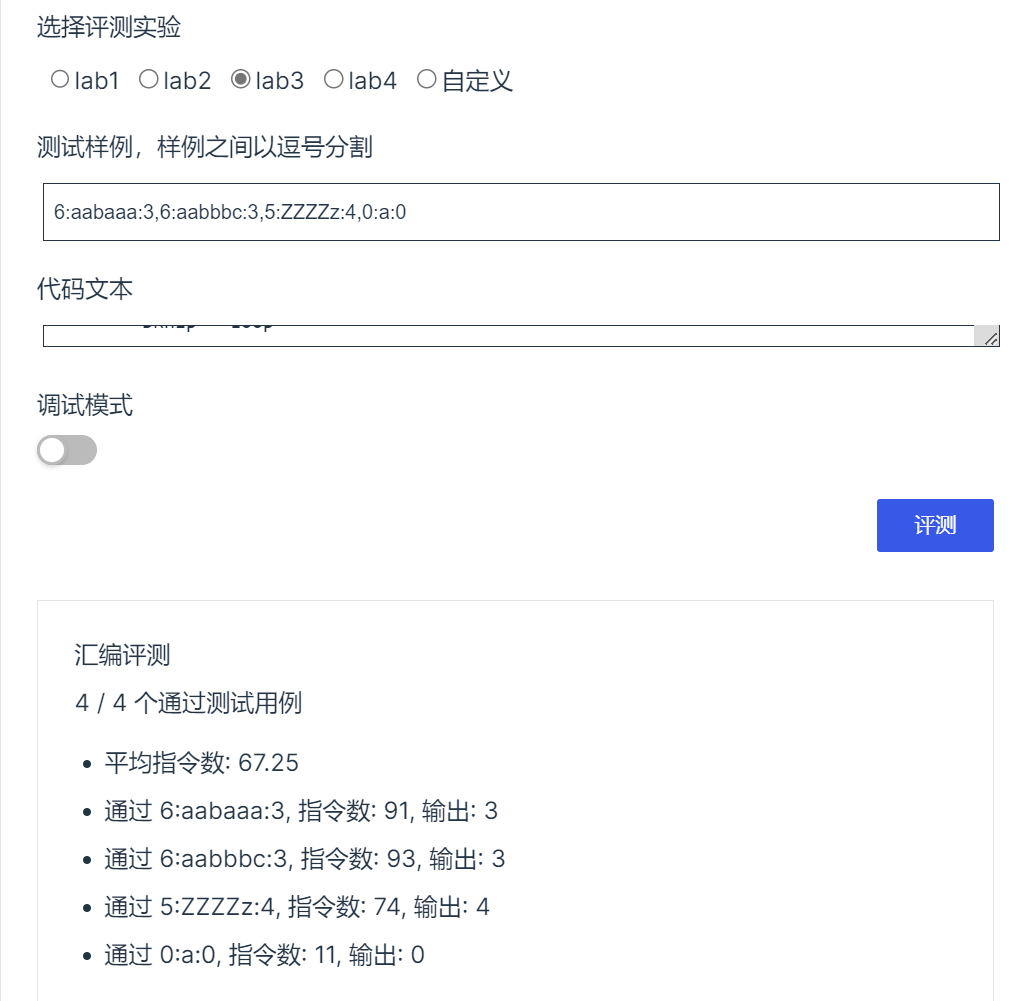
\includegraphics[scale=0.8]{r.png}
    \end{figure*}
\end{document}
\begin{lstlisting}[basicstyle=\ttfamily,language={[x86masm]Assembler}]

\end{lstlisting}